\section{Software}
Usa el paradigma del productor consumidor, tiene una aplicación que envía y otra que recibe.
\begin{itemize}	
	\item La aplicación de envío ofrece controles para elegir el dispositivo de llegada.
	\item La aplicación receptora utiliza una aplicación web ejecutada en un entorno de Chrome del dispositivo. Se pueden hacer aplicaciones receptoras que aparte de soportar HTML5 tengan más variedad de protocolos de streaming: MPEG-DASH, HTTP Live Streaming, y Microsoft Smooth Streaming Protocol.
\end{itemize}

Chromecast usa el protocolo mDNS (multicast Domain Name System) para buscar dispositivos disponibles en una red Wi-Fi, anteriormente usaba el protocolo DIAL (DIscovery And Launch).




\begin{figure}[ht] 
	\begin{minipage}[b]{0.55\linewidth}
	Utiliza un sistema operativo de escritorio llamado Chrome OS, siendo el navegador Google Chrome su principal herramienta de uso.  
	Chrome OS se basa en el proyecto de código abierto Chromium OS,5 que, a diferencia de Chrome OS, se puede compilar a partir del código fuente descargado.
	\end{minipage}%%
	\begin{minipage}[b]{0.45\linewidth}
		\centering
		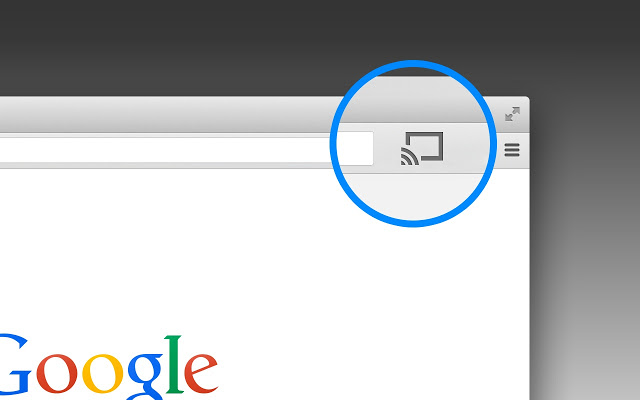
\includegraphics[width=.65\linewidth]{./Imagenes/googlecastbrowser.jpg} 
	\end{minipage} 
\end{figure}

\subsection{Google Cast}
\subsection{mDNS (multicast Domain Name System)}
\subsection{Miracast?}

\subsection{Chrome OS?}